Some definitions and results that are used throughout the text are given in this chapter.

\section{Elliptical and Euclidean norm functions}

A norm in $\R^2$ is a function that maps every vector onto a non-negative real number satisfying homogeneity and the triangle inequality. 

Let $u \in \R^2$ be a vector, the Euclidean norm of $u$ is defined as

\begin{equation*}
||u||_2 = \sqrt{u^{T}u}.
\end{equation*}
The elliptical norm, also known as weighted norm, takes a $2$ by $2$ positive definite matrix as its parameter. This matrix can be seen as a linear transformation of the Euclidean norm. The elliptical norm of $u \in\R^2$ is defined as 

\begin{equation*}
||u||_{Q} = \sqrt{u^{T}Qu},
\end{equation*}
where $Q$ is a $2$ by $2$ positive definite matrix. Note that the elliptical norm, when taking $Q$ to be the identity matrix, becomes the Euclidean norm.

Determining the distance between two points, given a norm function, is done by calculating the norm of the vector defined by the difference between the two points. For example, the elliptical distance between the points $p,q \in \R^2$ is given by $||p-q||_{Q}$.

\section{Disk}

A circle (or circumference) is a set of points in $\R^2$ that have the same Euclidean distance, also known as radius, to another point, also referred to as the center of the circle. A unit circle is a circle with radius equal to $1$.

A disk is the set of points bounded by a circle. In other words let $c \in \R^2$. A unit disk with center $c$ is the set of every point $p \in \R^2$ which satisfies

\begin{equation}\label{eq:disk}
||p-c||_2^2 \le 1.
\end{equation} 

\section{Ellipse}

An ellipse is a curve which is categorized, along with the parabola and the hyperbola, as a conic section. 
They get this name because conic sections are curves resulted from the intersection of a right circular cone in $\R^3$ with a plane \cite{brannan:geometry}. From that definition, an equation which describes any conic section is given as follows
\begin{equation}\label{equation:quadratic_form}
Ax^2 + Bxy + Cy^2 + Dx + Ey + F = 0,
\end{equation}
where $A,B,C,D,E,F \in \R$ are fixed and $x, y \in \R$. Distinguishing an ellipse from the other conic sections can be done using the condition
\begin{equation*}
4AC - B^2>0.
\end{equation*}
More details about conic sections can be found in \citeonline{ayoub}.

Assuming the center of an ellipse is $c \in \R^2$, then \autoref{equation:quadratic_form} can be rewritten as a quadratic form as follows
\begin{equation*}
(p-c)^{T}Q(p-c) = 1,
\end{equation*}
with $p \in \R^2$ and $Q$ being a $2$ by $2$ positive definite matrix which carries the parameters of the ellipse. From \autoref{equation:quadratic_form}, $Q$ can be defined as follows
\[
Q=
\left( {\begin{array}{cc}
	A & \frac{B}{2} \\
	\frac{B}{2} & C \\
	\end{array} } \right).
\]
Note that asking $Q$ to be positive definite is the same as asking $4AC-B^2$ to be positive. This makes us arrive at the following definition of the ellipse.

\begin{definicao}\label{def:ellipse}
    Let $c\in \R^2$ be the center of an ellipse and $Q$ be a $2$ by $2$ positive definite matrix. An ellipse is the set of every point $p \in \R^2$ such that $||p-c||_{Q}^2 = (p-c)^{T}Q(p-c) = 1$. Also, a point $p$ is considered covered by an ellipse if $||p-c||_{Q}^2 = (p-c)^{T}Q(p-c) \le 1$.
\end{definicao}

An alternative way to define an ellipse, which can be seen as just a property derived from the definition above, is to begin its construction with two points called foci and a constant $R \in \R$, with $R$ being greater than the Euclidean distance between the two foci points (see \autoref{fig:ellipse_with_foci}). The ellipse is, then, defined as the set of points whose distance to the foci is equal to $R$. In other words, let $f_1, f_2 \in \R^2$ be the two foci points, the ellipse is the set of every point $p \in \R^2$, such that $||p-f_1||_2 + ||p-f_2||_2 = R$. It can be shown that this definition is equivalent to \autoref{def:ellipse}, with the coverage of a point $p$ being equivalent to $||p-f_1||_2 + ||p-f_2||_2 \le R$.

\begin{figure}[H]
    \centering
    
    \caption{A non-axis-parallel ellipse and its foci points.}
    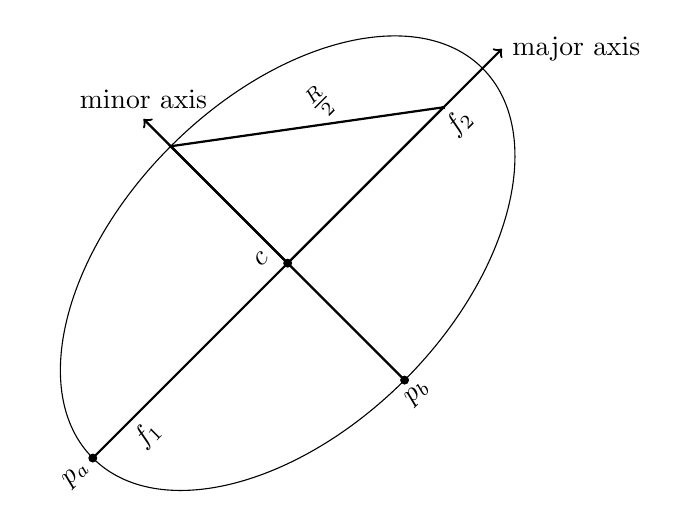
\begin{tikzpicture}[xscale=0.7, yscale=0.7][domain=0:11]
   % \draw [help axis] (-5,-3) grid (5,3);

    \begin{scope}[rotate=45]
    \draw (0,0) ellipse (5cm and 3cm);
    \node[rotate=45][below] at (-4,0) {$f_1$};
    \node[rotate=45][below] at (4,0) {$f_2$};
    \draw[fill] (-4,0) circle [radius=.5pt];
    \draw[fill] (4,0) circle [radius=.5pt];
    \draw [thick] (4,0) -- (0,0) -- (0,3) -- (4,0);
    \draw[->,thick] (-5,0)--(5.5,0) node[right]{major axis};
    \draw[->,thick] (0,-3)--(0,3.7) node[above]{minor axis};
        \node[rotate=45] [left] at (0,0.4) {$c$};
    \node [rotate=45][right] at (2.1,1.65) {$\frac{R}{2}$};
    
   
    \node [rotate=45][left] at (-5,0) {$p_a$};
    \draw[fill] (-5,0) circle [radius=2pt];
    
        \draw[fill] (0,0) circle [radius=2pt];
    
    \draw[fill] (0,-3) circle [radius=2pt];
    \node [below][rotate=45] at (0,-3) {$p_b$};
    \end{scope}

    %a^2-b^2=c^2 -> c^2=25-9=16 -> c=4
    
    %\draw[fill] (0,0) circle [radius=.5pt];
	
    %
    %\draw[fill] (5,0) circle [radius=1pt];
    %\draw[fill] (0,3) circle [radius=1pt];
    %
    

    %\node [below] at (2.1,0) {$c$};
	%\node [left] at (-0.1,1.5) {$b$};



    %\node [above] at (5,0) {$(x_0+a,y_0)$};
    %\node [above] at (-5,0) {$(x_0-a,y_0)$};
    %\node [above] at (0,3) {$(x_0,y_0+b)$};
    %
    

    
    %\draw [-] (-5,0) -- (5,0);
     %\draw [-] (0,-3) -- (0,3);
     %\draw [|-|] (0.001,-0.1) -- (4.999,-0.1);
\end{tikzpicture}
    \fautor
    \label{fig:ellipse_with_foci}
\end{figure}

Also, in \autoref{fig:ellipse_with_foci}, the distance $a = ||p_a - c||_2$, where $p_a$ is one of the intersection points of the ellipse with the major axis, is called the semi-major, and the distance $b = ||p_b-c||_2$, where $p_b$ is one of the intersection points of the ellipse with the minor axis, is called the semi-minor. These two values are also referred to as the shape parameters of an ellipse.
Finally, an ellipse is said to be axis-parallel if its major axis (see \autoref{fig:ellipse_with_foci}), which is the line that passes through its two foci points, is parallel to the $x$-axis.

\subsection{Axis-parallel ellipse}

An axis-parallel ellipse centered at $c = (c_x,c_y)$ can be described using \autoref{def:ellipse} with $Q$ being a diagonal matrix \footnote{The only non-zero terms are in the main diagonal.}. This can be understood as a scaling transformation applied to the Euclidean norm.

Defining the matrix $Q$ as

\[
Q=
\left( {\begin{array}{cc}
    \frac{1}{a^2} & 0 \\
    0 & \frac{1}{b^2} \\
    \end{array} } \right),
\]
then, starting from \autoref{def:ellipse}, we can obtain the following equation

 \begin{align}\label{equation:pellipse}
 (p-c)^{T}Q(p-c) &= 1 & \Rightarrow \nonumber \\
 (\frac{p_x-c_x}{a^2}, \frac{p_y-c_y}{b^2})^{T}(p_x-c_x, p_y-c_y) &= 1 & \Rightarrow \nonumber\\
  \frac{(p_x-c_x)^2}{a^2} + \frac{(p_y-c_y)^2}{b^2} &= 1,&
 \end{align}
where $(a, b) \in \R^2_{>0}$, with $a>b$, are ellipse's shape parameters.
Also, the coverage region is determined by just changing the equality to an inequality as follows
\begin{equation}\label{equation:cover_pellipse}
\frac{(p_x-c_x)^2}{a^2} + \frac{(p_y-c_y)^2}{b^2} \le 1.
\end{equation}

Another way to represent ellipses, which will be useful in some occasions, is through writing it as a curve function of the angle with its major axis (see \autoref{fig:ellipse_params}).

\begin{figure}[H]
    \centering
    
    \caption{The ellipse as a parametric curve.}
%    

%\tikzset{every picture/.style={line width=0.75pt}} %set default line width to 0.75pt        

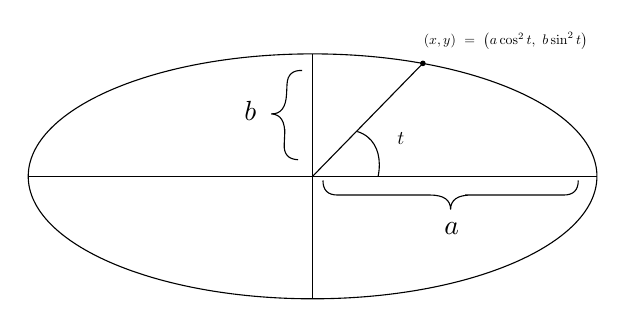
\begin{tikzpicture}[x=0.75pt,y=0.75pt,yscale=-1,xscale=1]
%uncomment if require: \path (0,300); %set diagram left start at 0, and has height of 300

%Shape: Ellipse [id:dp1559950964552308] 
\draw   (100,180) .. controls (100,147.42) and (161.34,121) .. (237,121) .. controls (312.66,121) and (374,147.42) .. (374,180) .. controls (374,212.58) and (312.66,239) .. (237,239) .. controls (161.34,239) and (100,212.58) .. (100,180) -- cycle ;
%Straight Lines [id:da3716259356733107] 
\draw    (100,180) -- (374,180) ;


%Straight Lines [id:da9880464900454329] 
\draw    (237,121) -- (237,239) ;


%Shape: Brace [id:dp3973633345998604] 
\draw   (242,182) .. controls (242,186.67) and (244.33,189) .. (249,189) -- (293.5,189) .. controls (300.17,189) and (303.5,191.33) .. (303.5,196) .. controls (303.5,191.33) and (306.83,189) .. (313.5,189)(310.5,189) -- (358,189) .. controls (362.67,189) and (365,186.67) .. (365,182) ;
%Shape: Brace [id:dp94498526835576] 
\draw   (232,129) .. controls (227.34,128.79) and (224.9,131.01) .. (224.68,135.67) -- (224.47,140.23) .. controls (224.16,146.89) and (221.68,150.11) .. (217.01,149.9) .. controls (221.68,150.11) and (223.85,153.55) .. (223.54,160.21)(223.68,157.21) -- (223.33,164.68) .. controls (223.12,169.35) and (225.34,171.79) .. (230,172) ;
%Shape: Arc [id:dp3154280429415799] 
\draw  [draw opacity=0] (258.54,158.43) .. controls (260.37,158.96) and (262.06,159.82) .. (263.54,161.03) .. controls (268.5,165.07) and (270.12,172.1) .. (268.62,179.79) -- (244.51,184.38) -- cycle ; \draw   (258.54,158.43) .. controls (260.37,158.96) and (262.06,159.82) .. (263.54,161.03) .. controls (268.5,165.07) and (270.12,172.1) .. (268.62,179.79) ;
%Shape: Circle [id:dp8908034615999807] 
\draw  [fill={rgb, 255:red, 0; green, 0; blue, 0 }  ,fill opacity=1 ] (289.08,125.57) .. controls (289.08,124.98) and (289.56,124.51) .. (290.14,124.51) .. controls (290.73,124.51) and (291.21,124.98) .. (291.21,125.57) .. controls (291.21,126.16) and (290.73,126.64) .. (290.14,126.64) .. controls (289.56,126.64) and (289.08,126.16) .. (289.08,125.57) -- cycle ;
%Straight Lines [id:da6323920079482996] 
\draw    (290.14,125.57) -- (237,180) ;



% Text Node
\draw (304,205) node   {$a$};
% Text Node
\draw (207,148.33) node   {$b$};
% Text Node
\draw (330,114.67) node [scale=0.5]  {$( x,y) \ =\ \left( a\cos^{2} t,\ b\sin^{2} t\right)$};
% Text Node
\draw (279.6,162) node [scale=0.7]  {$t$};


\end{tikzpicture}

   	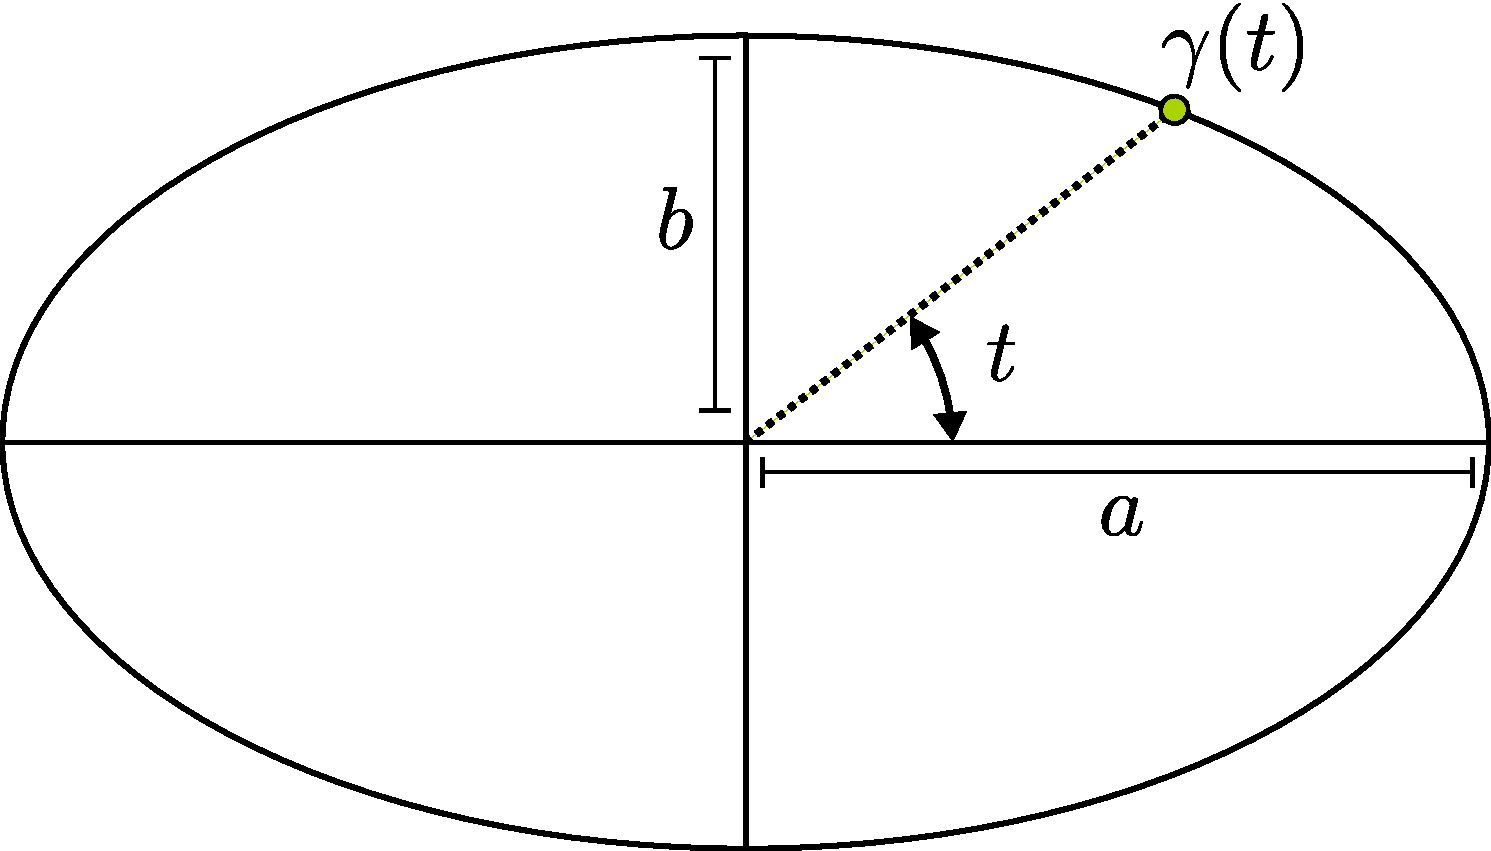
\includegraphics[scale=.36]{tex/figures/ellipse_definition.pdf}
    \fautor
    \label{fig:ellipse_params}
\end{figure}

Let $c \in \R^2$ be the center of an ellipse with shape parameters $(a,b) \in \R^2_{>0}$, with $a>b$. Then $\gamma\colon[0, 2\pi)\mapsto\R^2$ defines a curve which maps every angle onto a point on the ellipse and it is defined as follows
\begin{equation}\label{eq:parametric_ellipse}
\gamma(t) = \left\{
\begin{array}{l}
x(t)= a\cos{t} + c_x,\\
y(t)=b\sin{t} + c_y.
\end{array}
\right.
\end{equation}
Also, its derivative with respect to $t$ is given as follows
\begin{equation}\label{eq:der_parametric_ellipse}
\gamma'(t) = \left\{
\begin{array}{l}
x'(t)= -a\sin{t},\\
y'(t)=b\cos{t}.
\end{array}
\right.
\end{equation}

\subsection{The distance between points of an ellipse-line intersection}

Consider an ellipse with shape parameters $(a, b)\in\R^2_{>0}$, centered at the origin, and a line represented by the equation $y=mx+c$, with $m, c\in \R$. Suppose that this line intersects the ellipse at least at one point. Plugging the line's equation into \autoref{equation:pellipse}, it is possible to obtain the distance between the intersection points. The final expression is given by
\begin{equation*}\label{eq:dist_line_ellipse}
D(m, c)=\dfrac{\sqrt{(a^2m^2+b^2-c^2)(4a^2b^2(1+m^2))}}{(a^2m^2+b^2)},
\end{equation*}
with $D : \R^2 \mapsto \R_{\ge0}$ being a function of the line parameters $(m, c)$. It is also possible to see that, when $m$ is fixed, $D(m, c)^2$ is a parabola, and that $D(m, c)$ is maximized at $c=0$. From that, we can conclude that if $m$ is fixed, the line that has the most distant intersection points with an ellipse is the one that passes through the origin; and also, that $D(m, c)$ attains every value in the range $[0, D(m, 0)]$. 
Following that, we define a function $L:\R\mapsto\R_{>0}$ as

\begin{equation}\label{eq:function-l}
L(m):= D(m, 0)^2 = \dfrac{(a^2m^2+b^2)(4a^2b^2(1+m^2))}{(a^2m^2+b^2)^2},
\end{equation}
which describes the maximum distance between points of an ellipse-line intersection considering all lines with $m$ angular coefficient.

It is possible, by calculating the derivatives, to conclude that $L$ has its maximum at $m=0$, is increasing in $[0, \infty)$, is decreasing in $(-\infty\, 0]$, and attains every value in the interval $(4b^2, 4a^2]$. Notice that $L$ never hits $4b^2$ because that is the distance between the intersection of the ellipse with a vertical line.
In \autoref{fig:L-function-plot}, an example of function $L$ is shown with $(a, b) = (2, 1)$.

\begin{figure}[H]
	\centering
	
	\caption{Plot of function $L$ in the interval $[-7, 7]$.}
	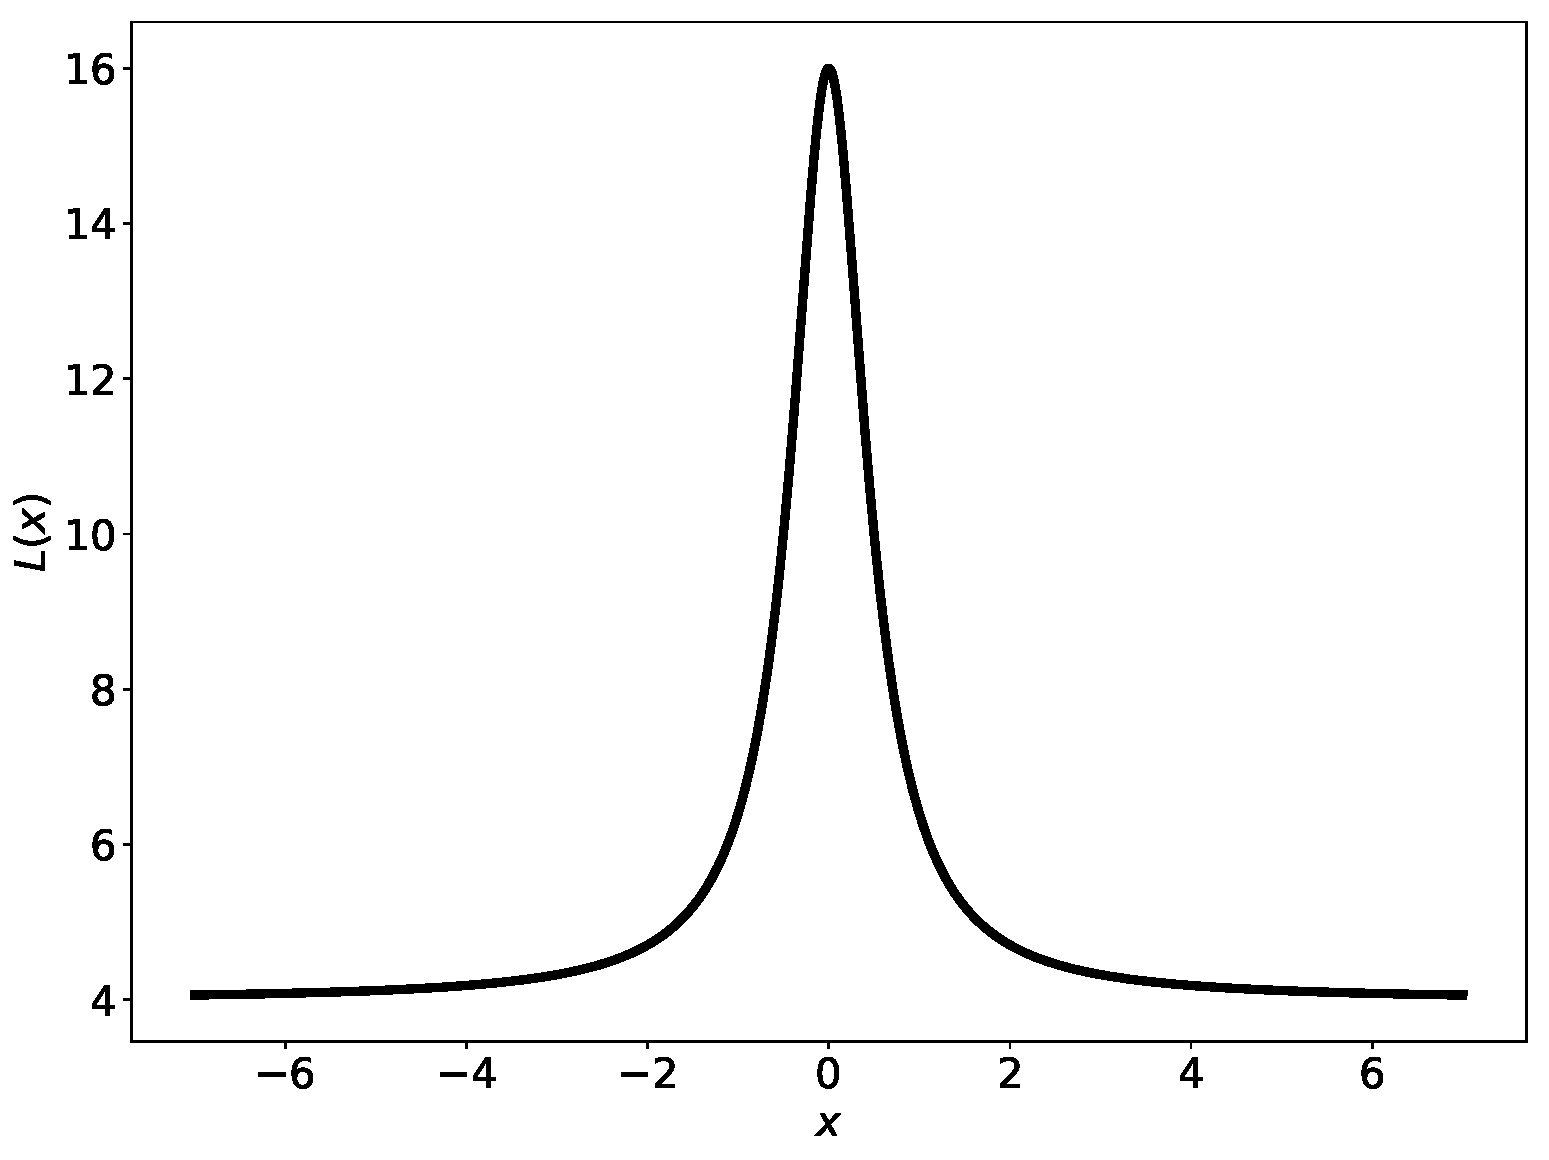
\includegraphics[scale=.4]{tex/figures/L-function-plot}
	\fautor
	\label{fig:L-function-plot}
\end{figure}

\subsection{Non-axis-parallel ellipse}

A non-axis-parallel ellipse centered at $(c_x, c_y)\in\R^2$ can also be described by \autoref{def:ellipse}, nonetheless, in this work,  a simpler equation is used instead. 
Besides the center and the shape parameters $(a, b) \in \R^2_{>0}$, with $a > b$; an angle of rotation $\theta \in \R$ is given representing the angle between the $x$-axis and the major axis of the ellipse. This can be seen on \autoref{fig:rotated_ellipse}, where the dashed lines represent the ellipse's axes and the angle between the major-axis and the $x$-axis is displayed.

An ellipse rotated by $\theta$ can be transformed into an axis-parallel, and origin-centered ellipse by applying two linear transformations: translation to make its center be at $(0, 0)$, and rotation to make its major axis parallel to the $x$-axis. Reversing these transformations produces the following equation for a non-axis-parallel ellipse
\begin{equation}\label{eq:rotated_ellipse}
\dfrac{((x-c_x)\cos\theta + (y-c_y)\sin\theta)^2}{a^2}+\dfrac{((x-c_x)\sin\theta - (y-c_y)\cos\theta)^2}{b^2}=1.
\end{equation}
The coverage region of that same ellipse is given by every point $(x, y)\in\R^2$ that satisfies the following equation
\begin{equation}\label{eq:rotated_ellipse_co}
\dfrac{((x-c_x)\cos\theta + (y-c_y)\sin\theta)^2}{a^2}+\dfrac{((x-c_x)\sin\theta - (y-c_y)\cos\theta)^2}{b^2}\le 1,
\end{equation}
which is the same as \autoref{eq:rotated_ellipse} with the equality sign $(=)$ replaced by $(\le)$.

Another important property of ellipses is shown on \autoref{fig:rotated_ellipse}. The two angles of rotation between the major axis and the $x$-axis ($\theta$ and $\theta+\pi$) are equivalent -- they produce the same ellipse. This symmetry is true for any angle of rotation, which means that $\theta$ is equivalent to $\theta+k\pi$, $k\in\mathbb{Z}$. Therefore, to represent any ellipse, it is enough to specify the domain of $\theta$ as $[0, \pi)$.

\begin{figure}[H]
	\centering
	
	\caption{The rotated ellipse.}
	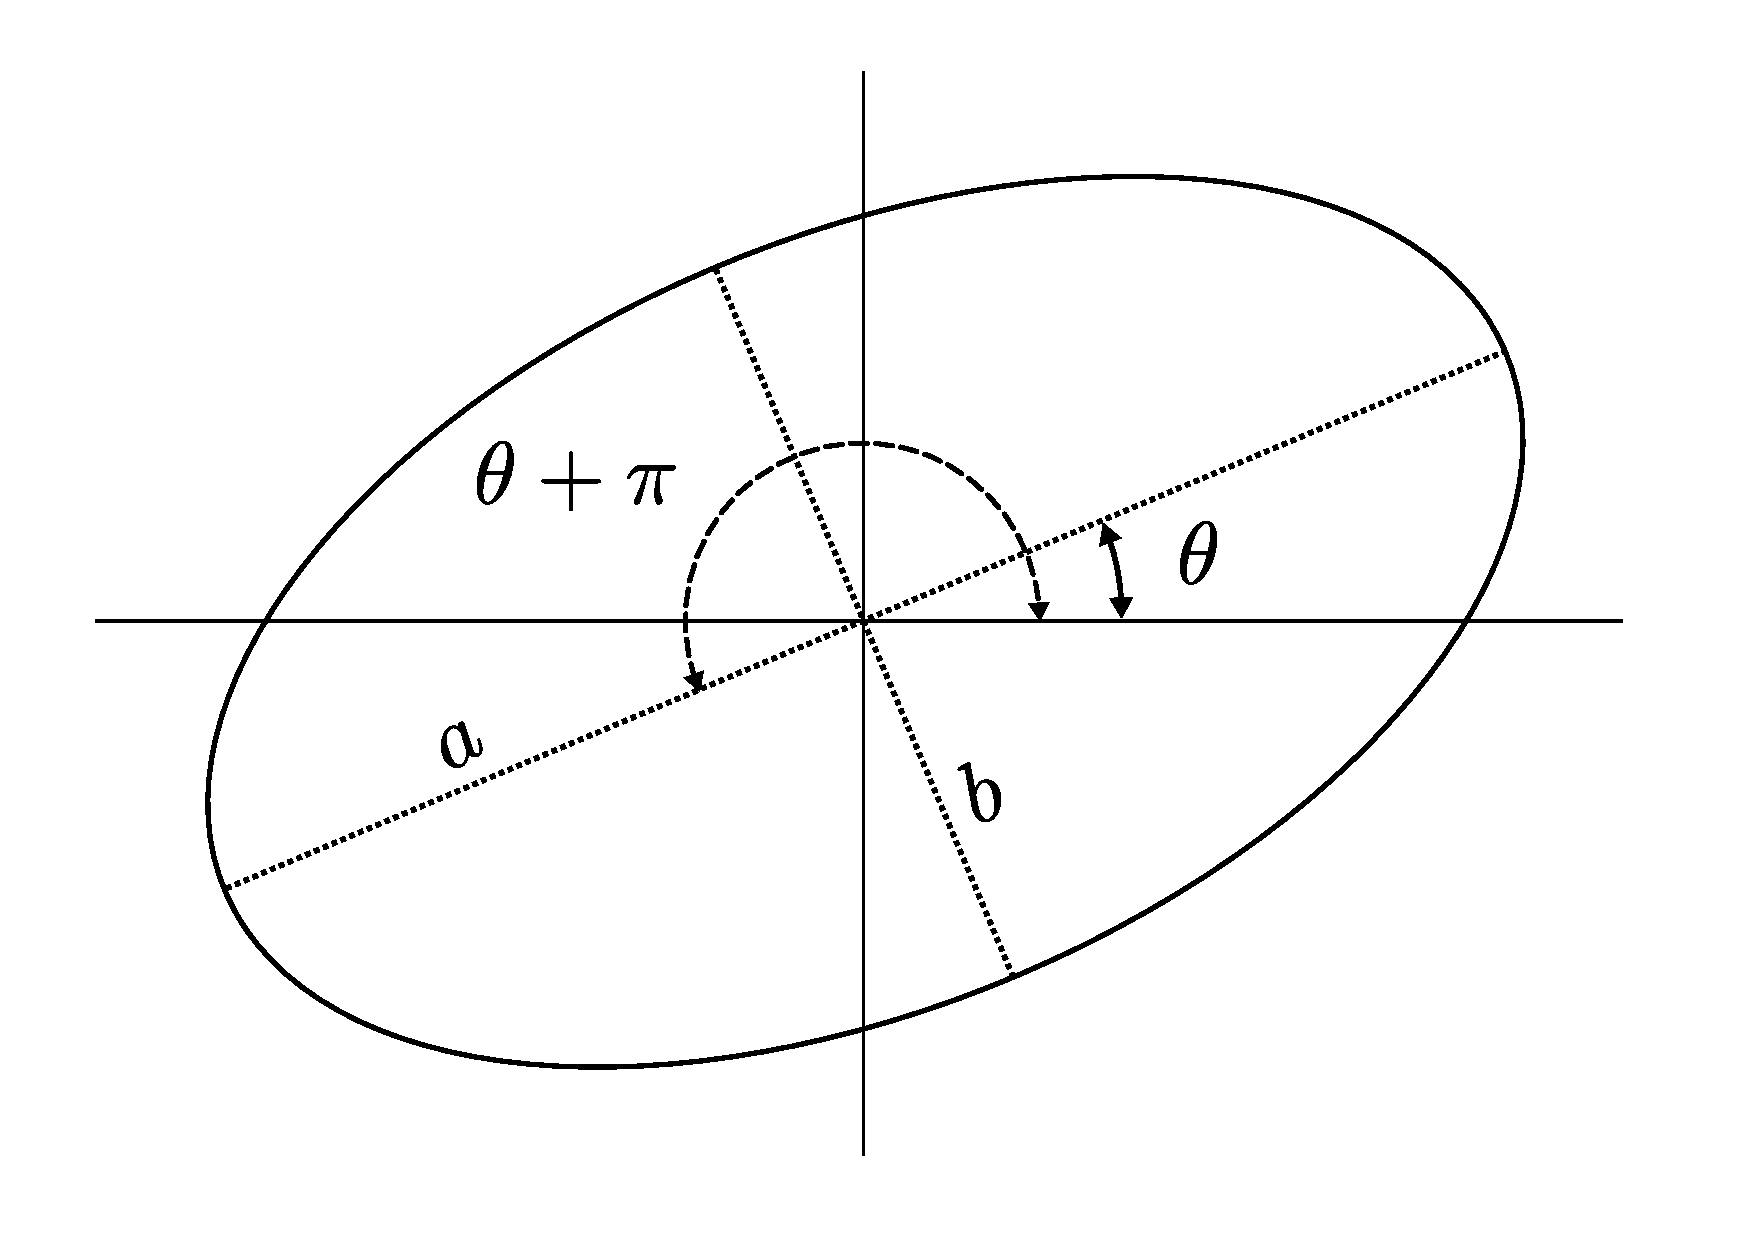
\includegraphics[scale=.38]{tex/figures/rotated_ellipse}
	\fautor
	\label{fig:rotated_ellipse}
\end{figure}


\subsection{Notation}

As stated by \autoref{def:ellipse}, the word ellipse is used to refer to the set of points that satisfies the equality equation, which can be seen as the border of an ellipse's coverage area. For this work, however, it is more convenient to refer directly to the coverage area of an ellipse and add a notation to express its border. For example, let $E$ be an ellipse's coverage area, and $\Pp \subset \R^2$ a set of points, then $E \cap \Pp$ denotes the set of points from $\Pp$ inside the coverage area of that ellipse. When we need to refer specifically to the border of $E$, we use the boundary operator: $\partial E$.


\section{Complex numbers}

The set of complex numbers $\mathbb{C}$ can be seen as just an extension of the set of real numbers $\R$. A thorough introduction on this topic is out of the scope and we just go through some basic properties that are going to be used later in \autoref{chapter:e3p}.

Any complex number $z\in\mathbb{C}$ is composed of a real part $a\in\R$, and an imaginary part $b\in\R$, multiple of the imaginary unit $i = \sqrt{-1}$. This is expressed as $z=a+ib$. 
Because complex numbers are composed of two real numbers, mapping $\mathbb{C}$ to $\R^2$, as shown in  \autoref{fig:complex-numbers}, provides a good way to visualize the set of complex numbers. 
This is also a good way to visualize Euler's Formula. As it can be seen on \autoref{fig:complex-numbers}, any complex number can be written in terms of its radius and polar angle as

\begin{equation*}
z = re^{i\theta}=r(\cos{\theta} + i\sin{\theta}),
\end{equation*}
with $r$ being the length of the vector determined by the point $z$ on the complex plane and $\theta = angle(z)$ being its polar angle. Note that $angle$ is a function from $\mathbb{C}$ to $[0, 2\pi)$.
\begin{figure}[ht]
	\centering
	\def\svgwidth{\columnwidth}
	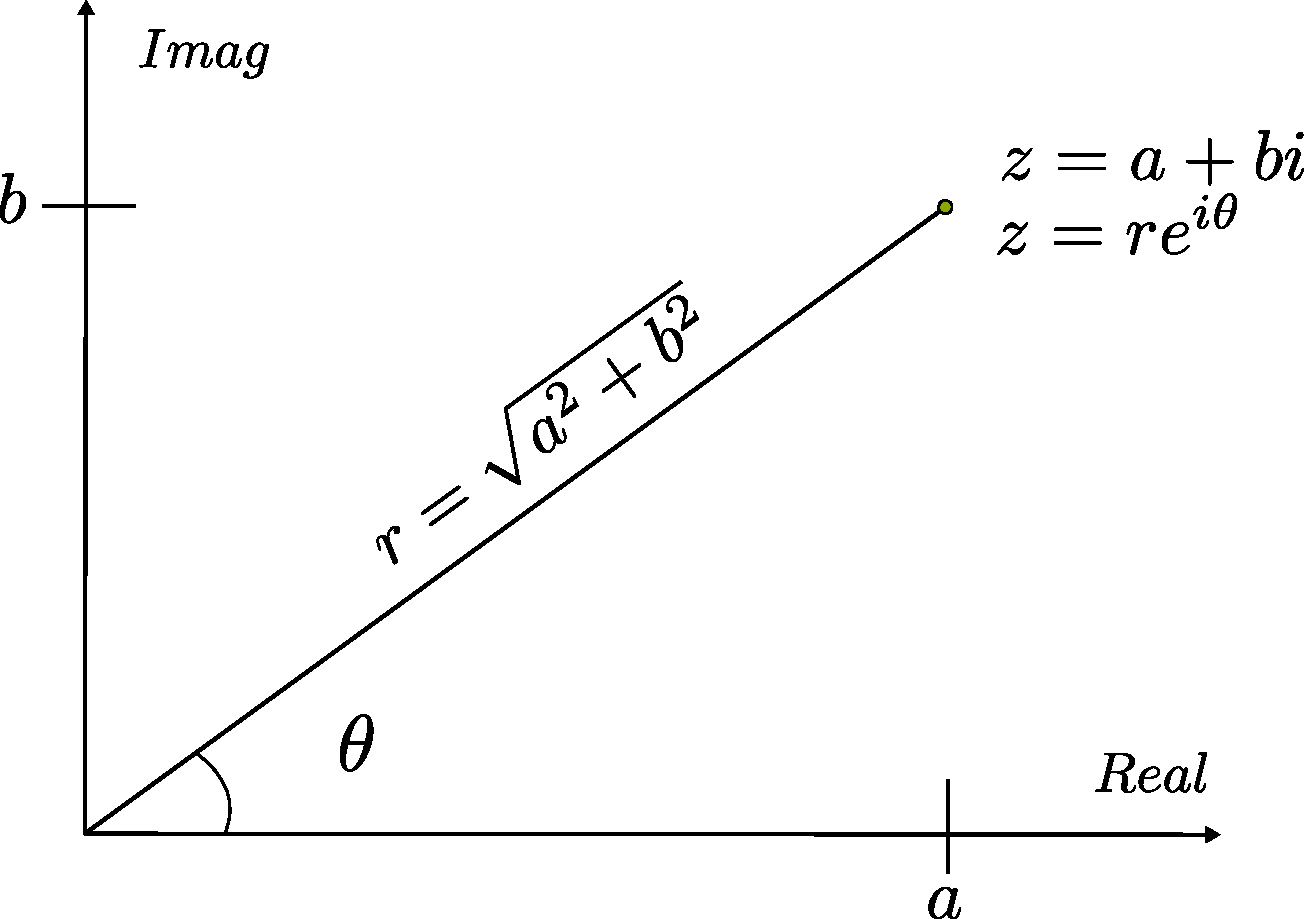
\includegraphics[scale=.37]{tex/figures/complex_numbers}
	\caption{The representation of a complex number on two dimensions.}
	\label{fig:complex-numbers}
\end{figure}

The complex conjugate is another important operator that is utilized later. Let $z = a + bi \in \mathbb{C}$, then we refer to $\bar{z}$ as the complex conjugate of $z$ and it is defined as
\begin{equation*}
\bar{z} = a - bi.
\end{equation*}
Lastly, two observations that are very important for the developments of \autoref{chapter:e3p} need to be stated. Let $z\in \mathbb{C}$, then we have 
\begin{align*}
angle(\bar{z}) = 2\pi-angle(z),\\
angle(-z) = \pi + angle(z).
\end{align*}
Checking the validity of these two equalities can be done by just observing the symmetry between the points defined by $z, \bar{z},$ and $-z$ on the plane.


\section{Polynomials and their roots}

In this work, we are mostly interested in univariate polynomials defined over the complex numbers.
A function $p_n: \mathbb{C} \mapsto \mathbb{C}$ is a $n$-degree polynomial if it can be written as
\begin{equation}\label{eq:poly}
p_n(z) = \sum_{k=0}^{n} a_k z^k,
\end{equation}
with $a_0, \dots, a_n \in \mathbb{C}$. In this work, when a polynomial is written in the form of \autoref{eq:poly} we say that it is in the power form or in the monomial form.

The famous Abel-Ruffini Theorem (a proof can be seen in \citeonline{skopenkov2015}) states that for polynomials of degree higher than four, there is no closed formula\footnote{A formula with a finite number of $+, -, \times, \div, \sqrt{}$.} to determine their roots. Fortunately, a numerical approach exists for higher-degree polynomials which works really well in practice.

 In \citeonline[p.~195]{horn} a theorem is presented which says that for every univariate polynomial of degree $n$, there exists a companion matrix which is a $n\times n$ matrix, such that its eigenvalues are the zeros of that polynomial. For example, the companion matrix of a degree-$5$ polynomial written as \autoref{eq:poly} is given by
 \begin{equation*}
 \left[\begin{array}{ccccc}
 0 & 1 & 0 & 0 & 0\\
 0 & 0 & 1 & 0 & 0\\
 0 & 0 & 0 & 1 & 0\\
 0 & 0 & 0 & 0 & 1\\
 -\dfrac{a_0}{a_5} & -\dfrac{a_1}{a_5} & -\dfrac{a_2}{a_5} & -\dfrac{a_3}{a_5} & -\dfrac{a_4}{a_5}
 \end{array}\right].
 \end{equation*}


Finding every eigenvalue of a matrix can be done using the QR algorithm, which runs in $\bigO(n^3)$ and uses $\bigO(n^2)$ memory (a very complete introduction to it can be found in \citeonline{watkins:2008}). 
The first step of the QR algorithm is to convert the input matrix into the Hessenberg form. This is done because matrices in the Hessenberg form maintain its form under the iterations of the algorithm. After that, the algorithm, under some assumptions, converges to the matrix's eigenvalues after $\bigO(n)$ iterations, each one taking $\bigO(n^2)$ computations.
Another method specific to companion matrices can be found in \citeonline{barel}. It uses the fact that companion matrices are already in the Hessenberg form to proposes a $\bigO(n^2)$ algorithm to find the roots of a $n$-degree polynomial.
 
 In practice, LAPACK's ZGEEV routine is utilized (the user guide can be found in \citeonline{lapack}), which is an implementation of the QR algorithm that returns every eigenvalue of a complex matrix.
 
\section{Real trigonometric polynomial}

The same definition found in \citeonline[p.~150]{powell} for real trigonometric polynomials is given here. They are also referred to as truncated Fourier Series in \citeonline{boyd:2006} and are given by
\begin{equation}\label{eq:trig_poly}
p_n(\theta) = \sum_{k=0}^{n} a_k\cos(k\theta) + \sum_{k=1}^{n} b_k\sin(k\theta).
\end{equation}
We say that $p_n: \R \mapsto \R$ as defined by \autoref{eq:trig_poly} is a $n$-degree real trigonometric polynomial. An important property is stated in \citeonline[p.~150]{powell}, which says that a $n$-degree polynomial can have up to $2n$ distinct roots on the interval $[0, 2\pi)$. It also says that a function written in the format
$$\begin{array}{cc}\cos^j{\theta}\sin^k{\theta}, & \quad j, k \in \mathbb{Z}_+, \end{array}$$
can be transformed into a real trigonometric polynomial of degree $j+k$. Therefore, for some $\{c_{j,k} \in \R: 0 \le j+k \le n\}$, the expression
\begin{equation}\label{eq:trig_poly_2}
\sum_{0 \le j+k \le n}c_{j,k}\cos^j{\theta}\sin^k{\theta},
\end{equation}
also represents a $n$-degree real trigonometric polynomial.